\documentclass{tufte-handout}\usepackage{graphicx, color}
%% maxwidth is the original width if it is less than linewidth
%% otherwise use linewidth (to make sure the graphics do not exceed the margin)
\makeatletter
\def\maxwidth{ %
  \ifdim\Gin@nat@width>\linewidth
    \linewidth
  \else
    \Gin@nat@width
  \fi
}
\makeatother

\definecolor{fgcolor}{rgb}{0.2, 0.2, 0.2}
\newcommand{\hlnumber}[1]{\textcolor[rgb]{0,0,0}{#1}}%
\newcommand{\hlfunctioncall}[1]{\textcolor[rgb]{0.501960784313725,0,0.329411764705882}{\textbf{#1}}}%
\newcommand{\hlstring}[1]{\textcolor[rgb]{0.6,0.6,1}{#1}}%
\newcommand{\hlkeyword}[1]{\textcolor[rgb]{0,0,0}{\textbf{#1}}}%
\newcommand{\hlargument}[1]{\textcolor[rgb]{0.690196078431373,0.250980392156863,0.0196078431372549}{#1}}%
\newcommand{\hlcomment}[1]{\textcolor[rgb]{0.180392156862745,0.6,0.341176470588235}{#1}}%
\newcommand{\hlroxygencomment}[1]{\textcolor[rgb]{0.43921568627451,0.47843137254902,0.701960784313725}{#1}}%
\newcommand{\hlformalargs}[1]{\textcolor[rgb]{0.690196078431373,0.250980392156863,0.0196078431372549}{#1}}%
\newcommand{\hleqformalargs}[1]{\textcolor[rgb]{0.690196078431373,0.250980392156863,0.0196078431372549}{#1}}%
\newcommand{\hlassignement}[1]{\textcolor[rgb]{0,0,0}{\textbf{#1}}}%
\newcommand{\hlpackage}[1]{\textcolor[rgb]{0.588235294117647,0.709803921568627,0.145098039215686}{#1}}%
\newcommand{\hlslot}[1]{\textit{#1}}%
\newcommand{\hlsymbol}[1]{\textcolor[rgb]{0,0,0}{#1}}%
\newcommand{\hlprompt}[1]{\textcolor[rgb]{0.2,0.2,0.2}{#1}}%

\usepackage{framed}
\makeatletter
\newenvironment{kframe}{%
 \def\at@end@of@kframe{}%
 \ifinner\ifhmode%
  \def\at@end@of@kframe{\end{minipage}}%
  \begin{minipage}{\columnwidth}%
 \fi\fi%
 \def\FrameCommand##1{\hskip\@totalleftmargin \hskip-\fboxsep
 \colorbox{shadecolor}{##1}\hskip-\fboxsep
     % There is no \\@totalrightmargin, so:
     \hskip-\linewidth \hskip-\@totalleftmargin \hskip\columnwidth}%
 \MakeFramed {\advance\hsize-\width
   \@totalleftmargin\z@ \linewidth\hsize
   \@setminipage}}%
 {\par\unskip\endMakeFramed%
 \at@end@of@kframe}
\makeatother

\definecolor{shadecolor}{rgb}{.97, .97, .97}
\definecolor{messagecolor}{rgb}{0, 0, 0}
\definecolor{warningcolor}{rgb}{1, 0, 1}
\definecolor{errorcolor}{rgb}{1, 0, 0}
\newenvironment{knitrout}{}{} % an empty environment to be redefined in TeX

\usepackage{alltt}

%\geometry{showframe}% for debugging purposes -- displays the margins
\usepackage[utf8]{inputenc}
\usepackage{amsmath}
\usepackage[spanish]{babel}
% Set up the images/graphics package
\usepackage{graphicx}
\usepackage{colortbl}
\setkeys{Gin}{width=\linewidth,totalheight=\textheight,keepaspectratio}
\graphicspath{{graphics/}}
%\usepackage[table]{xcolor}
% The following package makes prettier tables.  We're all about the bling!
\usepackage{booktabs}

% The units package provides nice, non-stacked fractions and better spacing
% for units.
\usepackage{units}

% The fancyvrb package lets us customize the formatting of verbatim
% environments.  We use a slightly smaller font.
\usepackage{fancyvrb}
\fvset{fontsize=\normalsize}

% Small sections of multiple columns
\usepackage{multicol}

% Provides paragraphs of dummy text
\usepackage{lipsum}

\title{Práctica gráfica en tesis de Actuaría (ITAM, 1990-2007)}
\author{Felipe González y grupo de Estadística Aplicada I, Otoño 2007}
\IfFileExists{upquote.sty}{\usepackage{upquote}}{}





\begin{document}
%\maketitle
%\normalsize
%\raggedright
%\setlength\parindent{10pt}


\maketitle

\begin{abstract}
Los métodos gráficos
son una herramienta poderosa en
el análisis de datos. En contraste con otros métodos,
sólo hasta recientemente han aparecido guías sólidas
(aunque todavía parciales)
de lo que constituye la buena práctica gráfica,
y estas guías son relativamente poco conocidas.

Un punto de partida para la difusión de estas guías
es el diagnóstico de la práctica actual, que varía
mucho según el contexto (periódicos, industria,
publicaciones científicas). 
En este
trabajo buscamos producir estimaciones de
varios indicadores básicos para las tesis de Actuaría
en el periodo 1990-2007: qué tanto y qué tipos
de gráficas se usan, y 
algunos indicadores de la calidad de la práctica gráfica.


\end{abstract}





\subsection{Resultados principales y Recomendaciones}


Mostramos que las gráficas son
utilizadas comunmente en las tesis de actuaría (en particular
las de dispersión y las de barras),
y que podrían mejorar en varios aspectos: 

\begin{enumerate}
\item Reduciendo la basura gráfica en particular rejillas y rellenos,
\item Eliminando el uso de gráficas de pay, reduciendo el uso de gráficas
de barras y sustituirlas por gráficas de puntos o tablas.
\item Usando más ampliamente gráficas de páneles múltiples (pequeños
múltiplos).
\end{enumerate}


\subsection{La mayor parte de las tesis de Actuaría requieren presentar datos
en forma gráfica o tabular}


Diferentes tesis, por su naturaleza, requieren de más o menos representaciones
de datos, y la elección es utilizar gráficas o tablas. 
El 95\% ${\pm 3}$\% de las tesis continen al menos una gráfica o una tabla,
y el 80\% ${\pm 6}$\% contiene
tanto gráficas como tablas.



Las dos gráficas de abajo sugieren que después de 2000 se ha incrementado
el uso y presentación 
de datos en las tesis de Actuaría (total de gráficas y tablas presentadas),
aún cuando la elección entre tablas y gráficas no ha cambiado (los estudiantes de actuaría deciden por tablas el  64\% ${\pm 5}$ \% de las veces. )

Estos resultados pueden indicar que aún cuando se usa más representaciones de datos,
estas representaciones no han aumentado en tamaño o complejidad, lo que usualmente
requiere de gráficas en vez de tablas. Otra posible explicación es que las
tablas cada vez se usan en situaciones donde gráficas serían más apropiadas.



\begin{figure}[!h]
\centering
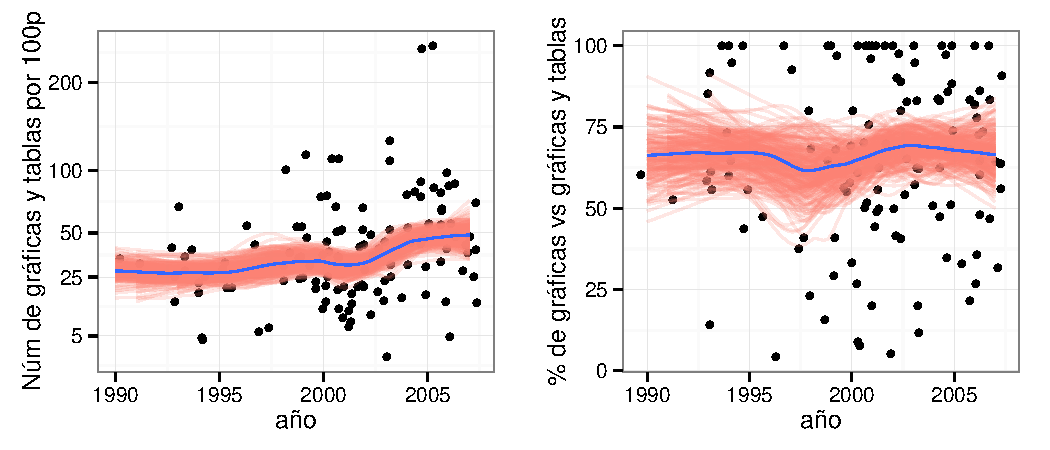
\includegraphics[width=12cm]{./figure/grafpor.pdf}
\caption{Graficas de datos y tablas por año. Bandas construidas con 200 replicaciones
bootstrap de un suavizamiento loess.}
\end{figure}








%\newgeometry{bottom=0.1cm}

 Alrededor del 84\% $\pm 6$ de las tesis de actuaría
 contiene por lo menos alguna gráfica de datos.
  El número de gráficas por cada cien páginas
 es de $18\pm3$, y  
  el 90\% de las tesis
 con más gráficas utilizan gráficas de manera intensiva
 (más de $[27,50]$ gráficas por cada cien páginas. 
 Abajo mostramos los cuantiles estimados, con algunas referencias más o menos conocidas.
 \sidenote[][3cm]{Cleveland, William S., {\it The Elements of
Graphing Data}, Hobart Press, 1994.


\vspace{\baselineskip}

{Venables, W.N. y Ripley, B.D., {\it Modern
 Applied Statistics with S-PLUS}, Springer, 2002.}

\vspace{\baselineskip}

{Pole A., West M. y Harrison, J., 
{\it Applied Bayesian Forecasting and Time Series
Analysis}, Chapman \& Hall, 1994.}

\vspace{\baselineskip}

{Hoaglin, D.C., Mosteller, F. y Tukey, J.W.,
{\it Understanding Robust and Exploratory Data Analysis},
Wiley, 1983.}

\vspace{\baselineskip}

{Rossi, P.E., Allenby, G. y McCulloch, R.,
{\it Bayesian Statistics and Marketing}, Wiley, 2005.}

\vspace{\baselineskip}

{Klugman, S. A., {\it Loss Models: From Data to Decisions},
Wiley-Interscience, 2004.}
} 


\begin{figure}[!h]
\caption{Deciles estimados de número de gráficas de datos.}

\centering
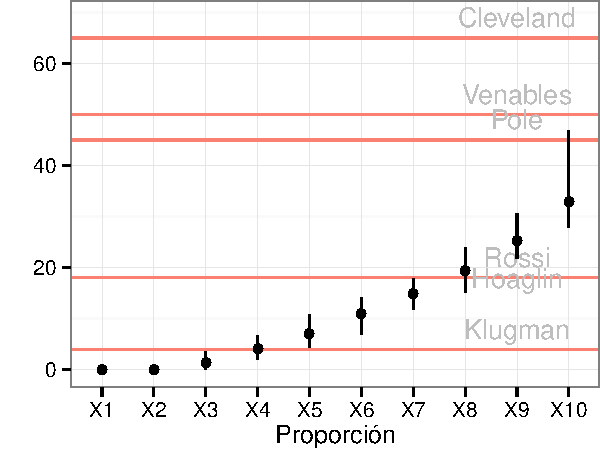
\includegraphics[width=6cm]{./figure/graf1.pdf}
\end{figure}


%Donde vemos también que no hay una relación simple entre
%el número de páginas y la densidad gráfica, aunque
%la gráfica de la izquierda suguiere que las tesis con
%densidades atípicamente altas tienden a ser cortas.

Los tres casos que tienen densidad gráfica mayor
al libro de Cleveland son interesantes: el mayor,
con 123 gráficas por 100 páginas (IAC-2005-EAR, 
{\it Análisis comparativo del nivel de religiosidad en estudiantes católicos de dos universidades...})
contiene algunas gráficas de barras y muchas gráficas de pay decorativas 
acompañadas de tablas de datos (que es el estilo
usual de la graficación de datos en la mercadotecnia). El segundo
(IAC 2003.RRI) es un dato atípico por varias razones: se trata de una
tesis de 31 páginas (sin contar bibliografía). Finalmente
tenemos IAC-1999-FAN, {\it Sistema Bonus-Malus 200 para
la conservación de la cartera}, que es atípica por el uso
extensivo de histogramas (para representar distribuciones de
pérdida).





\subsection{Tipos de gráficas}

Las gráficas más comunes son las dispersión (que no
son series de tiempo). En la siguiente tabla  mostramos
nuestras estimaciones para varias tipos de gráficas que
fueron medidos para la población de tesis que tienen al
menos una gráfica de datos.  





%\begin{margintable}
% latex table generated in R 3.0.0 by xtable 1.7-1 package
% Fri Jun 14 15:25:38 2013
\begin{table}[ht]
\centering
\begin{tabular}{rlrrrr}
  \hline
 & tipo & \% de gráficas &  & \% de tesis &  \\ 
  \hline
1 & Dispersión & 28 & \textcolor{gray}{ 3 } & 68 & \textcolor{gray}{ 4 } \\ 
  2 & Barras & 25 & \textcolor{gray}{ 3 } & 51 & \textcolor{gray}{ 4 } \\ 
  3 & Serie de tiempo & 24 & \textcolor{gray}{ 4 } & 52 & \textcolor{gray}{ 4 } \\ 
  4 & Histograma & 9 & \textcolor{gray}{ 2 } & 24 & \textcolor{gray}{ 4 } \\ 
  5 & Circular & 9 & \textcolor{gray}{ 3 } & 17 & \textcolor{gray}{ 3 } \\ 
  6 & Caja y brazos & 2 & \textcolor{gray}{ 1 } & 9 & \textcolor{gray}{ 2 } \\ 
  7 & Mapas & 1 & \textcolor{gray}{ 1 } & 4 & \textcolor{gray}{ 2 } \\ 
  8 & Otras & 0 & \textcolor{gray}{ 0 } & 2 & \textcolor{gray}{ 1 } \\ 
   \hline
\end{tabular}
\end{table}


%\end{margintable}

\vspace{1cm}
Las gráficas de barras son probablemente sobreutilizadas, y podrían sustituirse
con otro tipo o con tablas. El uso de pays es considerable.


Existen claras correlaciones entre la aparición de distintos tipos
de gráficas dependiendo de la tesis: a grandes rasgos, las gráficas de
barras y circulares tienden a aparecer juntas: son tesis que podrían parecer
presentaciones de {\em marketing}. Por otra parte, tenemos también algunas tesis
que utilizan gráficas más comunes en la estadística, como histogramas
y gráficas de dispersión:

\begin{marginfigure}[14cm]
  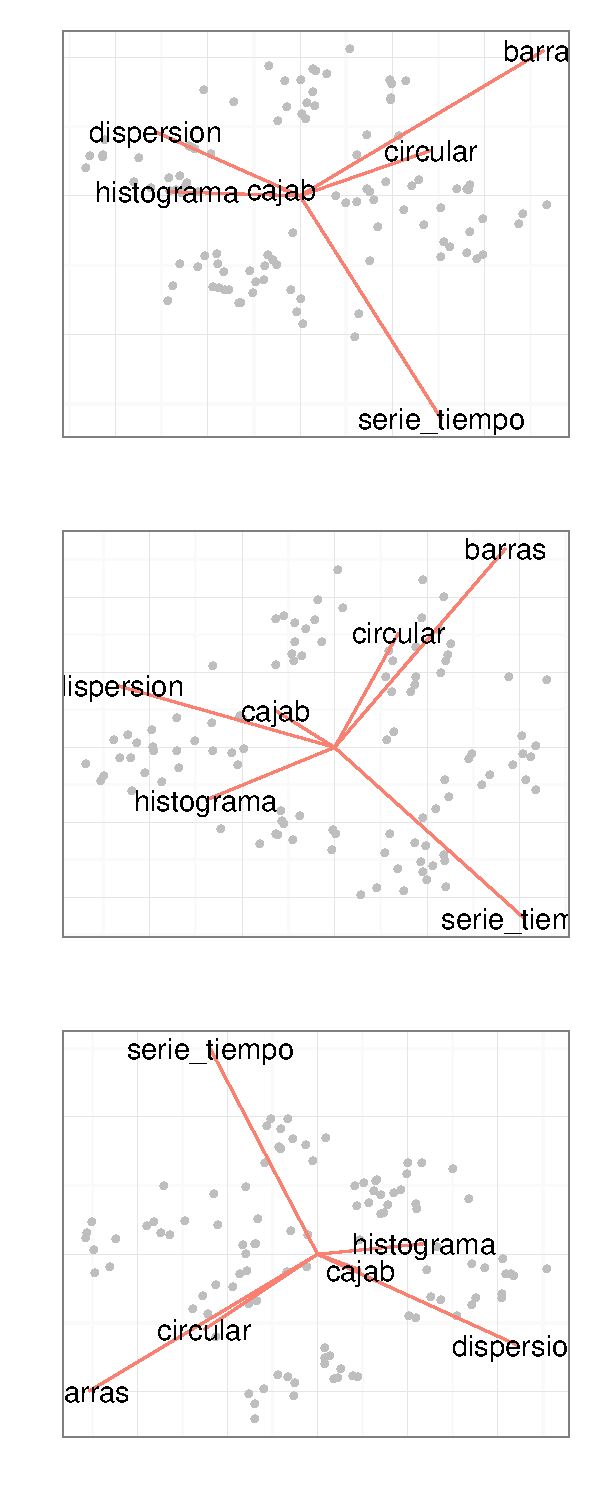
\includegraphics[width=3cm]{./figure/graf3.pdf}
  \caption{Replicaciones bootstrap de la gráfica de la izquierda}
\end{marginfigure}



\begin{figure}[!h]
\centering
\caption{Biplot de primeras dos componentes principales para tabla binaria de tesis por tipo de gráficas}
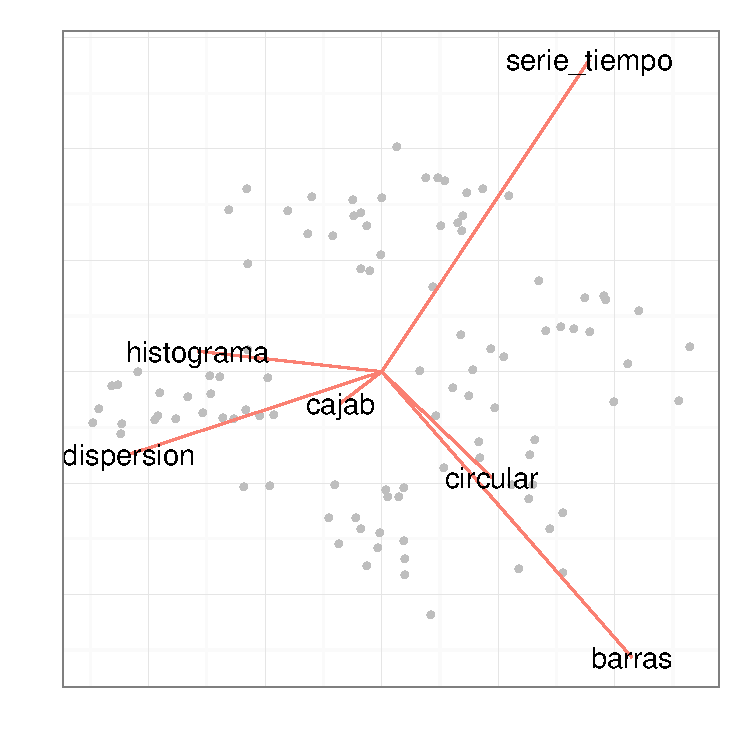
\includegraphics[width=7.5cm]{./figure/graf2.pdf}
\end{figure}














\subsection{Indicadores básicos de calidad gráfica}

En nuestro estudio tenemos dos indicadores básicos de la 
calidad de cada gráfica:
\begin{marginfigure}
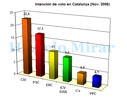
\includegraphics[width=3cm]{../doc/efecto_3d}
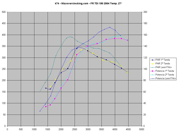
\includegraphics[width=3cm]{../doc/rejilla.png}
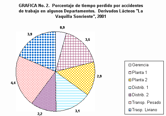
\includegraphics[width=3cm]{../doc/trama.png}
\caption{Tipos de basura gráfica: efecto 3d, rejilla, trama}
\end{marginfigure}

\begin{itemize}
\item Contenido de basura gráfica ({\em chartjunk} de Tufte, 
como efectos 3d, {\em grid} o rejillas
que ocultan o dificultan la percepción de los puntos de datos, marcos 
 superfluos, etc.).
\item Si la explicación de la gráfica está en la misma página de la gráfica o
no. En el mejor trabajo gráfico texto, tablas, diagramas y gráficas se
integran para explicar los datos.
\item Uso de pequeños múltiplos, que consisten en la replicación de un mismo
diseño y variando los datos en cada replicación.
\end{itemize}





%\begin{marginfigure}
%  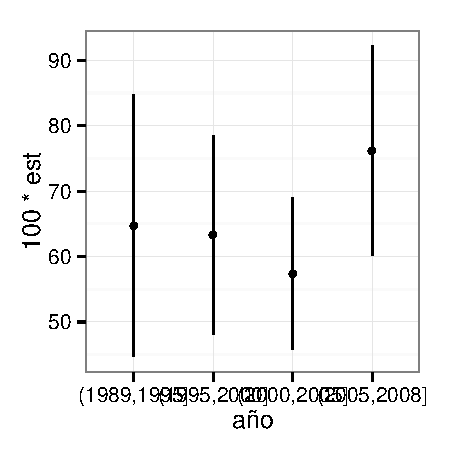
\includegraphics[width=4cm]{./figure/graftiempo.pdf}
%  \caption{\% de tesis con basura gráfica}
%\end{marginfigure}

Entre las tesis que contienen gráficas, el 75\%$\pm7$ contiene algún tipo
de basura gráfica, y el 47\% $\pm 7$ de las gráficas totales contiene algún
tipo de basura. Estos números indican que las tesis no se dividen claramente
en tesis sin basura y con basura.


Distintos tipos de basura gráfica están asociados a distintos tipos de gráficas:




\begin{figure*}
\centering
\caption{Tipos de basura gráfica registrados según tipo de gráfica. Los criterios
de basura gráfica son subjetivos (una rejilla se considera basura
si tiene un grosor y color similar a los datos graficados, por ejemplo). Gráfica sola indica que la gráfica no aparece junto a otra para comparar, y Sin explicación indica que la explicación de la gráfica se encuentra en otra página.}
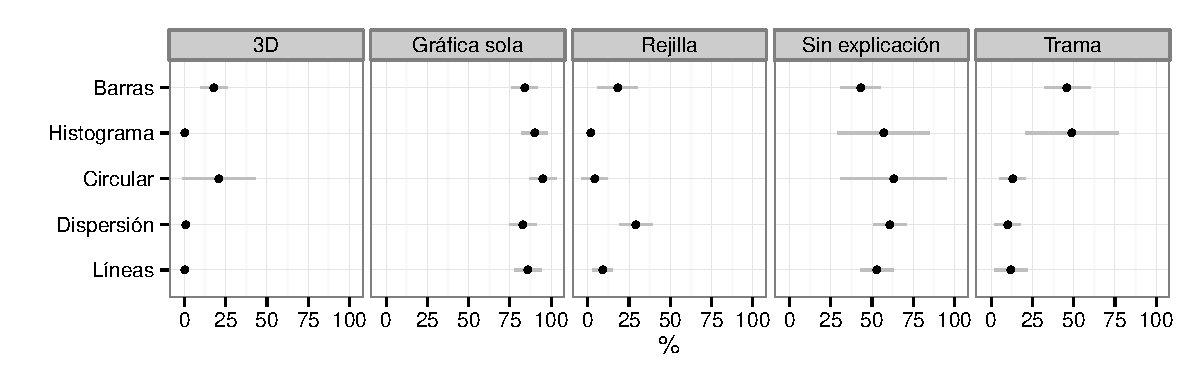
\includegraphics{./figure/grafbasura.pdf}
\end{figure*}







\subsection{Datos y diseño}

Se seleccionó una muestra aleatoria simple de tesis de Actuaría registradas
en la biblioteca con fecha entre 1990 y 2007 (Abril 2008). No se pudieron encontrar
3 de las 125 tesis seleccionadas en la muestra. Se registraron todas
las gráficas (separadas en gráficas de datos y gráficas analíticas según
criterios establecidos) contenidas en cada tesis seleccionadas, y cada
una se clasificó según su tipo y su contenido de basura gráfica. Los criterios
para basura gráfica son apreciativos: los estudiantes que levantaron los datos
fueron primero entrenados para regularizar en lo más posible los criterios.



\end{document}



